\paragraph{补充评注。}\label{sub:additional-remarks-17f}
\begin{figure}[htbp]
\centering
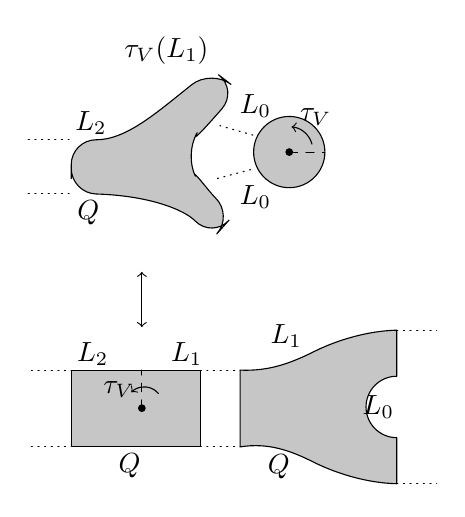
\begin{tikzpicture}[line cap=round,line join=round,scale=0.78]
\draw[dotted] (-0.7,1.05) -- (0,1.05);
\draw[dotted] (-0.7,0.18) -- (0,0.18);
\draw[fill=gray!45,rounded corners=9pt]
  (0,0.18) -- (0,1.05)
  .. controls (0.9,1.05) and (1.4,1.5) .. (2.28,2.2)
  -- (2.72,1.86)
  .. controls (2.1,1.15) and (1.95,1.0) .. (1.84,0.82)
  .. controls (1.95,0.6) and (2.25,0.2) .. (2.64,-0.18)
  -- (2.3,-0.56)
  .. controls (1.85,-0.1) and (1.3,0.14) .. (0,0.18) -- cycle;
\draw[dotted] (2.42,1.28) .. controls (2.7,1.2) .. (2.98,1.12);
\draw[dotted] (2.38,0.42) .. controls (2.68,0.5) .. (2.98,0.58);
\draw[fill=gray!45] (3.55,0.85) circle (0.58);
\fill (3.55,0.85) circle (1.8pt);
\draw[dashed] (3.55,0.85) -- (4.13,0.85);
\draw[->] (3.92,0.98) arc[start angle=15,end angle=85,radius=0.38];
\node at (1.55,2.5) {$\tau_V(L_1)$};
\node at (0.32,1.32) {$L_2$};
\node at (0.28,-0.14) {$Q$};
\node at (3.0,1.6) {$L_0$};
\node at (3.0,0.12) {$L_0$};
\node at (3.98,1.42) {$\tau_V$};
\draw[<->] (1.15,-1.1) -- (1.15,-2.0);
\draw[dotted] (-0.65,-2.7) -- (0,-2.7);
\draw[dotted] (-0.65,-3.95) -- (0,-3.95);
\draw[fill=gray!45] (0,-3.95) rectangle (2.1,-2.7);
\fill (1.15,-3.32) circle (1.8pt);
\draw[dashed] (1.15,-3.32) -- (1.15,-2.7);
\draw[->] (1.42,-3.08) arc[start angle=40,end angle=135,radius=0.3];
\node at (0.78,-3.02) {$\tau_V$};
\node at (0.35,-2.44) {$L_2$};
\node at (1.88,-2.44) {$L_1$};
\node at (0.95,-4.25) {$Q$};
\draw[dotted] (2.1,-2.7) -- (2.75,-2.7);
\draw[dotted] (2.1,-3.95) -- (2.75,-3.95);
\draw[fill=gray!45]
  (2.75,-2.7)
  .. controls (3.2,-2.72) and (3.55,-2.6) .. (3.95,-2.4)
  .. controls (4.35,-2.2) and (4.85,-2.06) .. (5.3,-2.05)
  -- (5.3,-2.8) arc[start angle=90,end angle=270,radius=0.5] -- (5.3,-4.55)
  .. controls (4.85,-4.54) and (4.35,-4.4) .. (3.95,-4.2)
  .. controls (3.55,-4.0) and (3.2,-3.88) .. (2.75,-3.95) -- cycle;
\draw[dotted] (5.3,-2.05) -- (5.95,-2.05);
\draw[dotted] (5.3,-4.55) -- (5.95,-4.55);
\node at (3.5,-2.14) {$L_1$};
\node at (3.38,-4.28) {$Q$};
\node at (5.0,-3.3) {$L_0$};
\end{tikzpicture}
\caption{}\label{fig:l-families}
\end{figure}
如同前面那样，我们同样可以证明：在定义 $(d,l)$ 时所涉及的那些选取本质上是无关紧要的。更确切地说，如果 $(d,l)$ 与 $(\tilde{d},\tilde{l})$ 是用不同的选取定义出来的，那么我们可以考虑一些额外的\trModuliSpace{}来在构造的这两个版本之间进行过渡，从而得到
\begin{equation*}
\boxed{\begin{aligned}
&\delta\colon CF^{\mathrm{pr}}(Q,L_1)\longrightarrow CF^{\mathrm{pr}}(Q,L_2),\\
&\lambda\colon CF^{\mathrm{pr}}(L_0,L_1)\otimes CF^{\mathrm{pr}}(Q,L_0)\longrightarrow CF^{\mathrm{pr}}(Q,L_2),\\
&\mu^1(\delta(\cdot))+\delta(\mu^1(\cdot))+d+\tilde{d}=0,\\
&\delta(\mu^2(\cdot,\cdot))+\mu^1(\lambda(\cdot,\cdot))+\lambda(\mu^1(\cdot),\cdot)+\lambda(\cdot,\mu^1(\cdot))+l+\tilde{l}=0.
\end{aligned}}
\end{equation*}
其代数意义是：我们由此得到\trChainComplex{} \eqref{eq:auxiliary-complex-differential} 之间的一个\trIsomorphism
\begin{equation}\label{eq:chain-complex-isomorphism-17f}
\begin{pmatrix}
\mathrm{Id}\otimes\mathrm{Id} & & \\
0 & \mathrm{Id} & \\
\lambda & \delta & \mathrm{Id}
\end{pmatrix}
\colon D\longrightarrow\tilde{D}.
\end{equation}
更一般地，我们可以考察 $(d,l)$ 如何依赖于 $L_1$。设 $\tilde{L}_1$ 是\trIsotopy{}于 $L_1$ 的另一个\trSubmanifold，并取与之相伴的版本 $(\tilde{d},\tilde{l})$。取\trContinuationMap
\begin{equation*}
\begin{gathered}
a\colon CF^{\mathrm{pr}}(Q,L_1)\longrightarrow CF^{\mathrm{pr}}(Q,\tilde{L}_1),\\
b\colon CF^{\mathrm{pr}}(L_0,L_1)\longrightarrow CF^{\mathrm{pr}}(L_0,\tilde{L}_1);
\end{gathered}
\end{equation*}
这些映射与\trTriangleProduct{}在\trChainHomotopy{}的意义下\trCompatible，也就是说，存在一个 $h\colon CF^{\mathrm{pr}}(L_0,L_1)\otimes CF^{\mathrm{pr}}(Q,L_0)\to CF^{\mathrm{pr}}(L_0,\tilde{L}_1)$ 使得
\begin{equation*}
\mu^1(h(\cdot))+h(\mu^1(\cdot),\cdot)+h(\cdot,\mu^1(\cdot))+\mu^2(b(\cdot),\cdot)+a(\mu^2(\cdot,\cdot))=0.
\end{equation*}
从我们的普遍观点来看，这些\trContinuationMap{}来自那些平凡\trFibration{}$M\times Z\to Z$：其\trBoundaryCondition{}在 $\RR\times\{0\}$ 之上是常值的且等于 $Q$ 或 $L_0$，而在 $\RR\times\{1\}$ 之上实现从 $\tilde{L}_1$ 到 $L_1$ 的\trIsotopy（这一点在 \cref{sub:tqft-definition} 中已经被指出过了）。我们可以取三\trPointedDisc{}上的一个平凡\trFibration，为其配备\trBoundaryCondition{}$(Q,L_0,L_1)$，并把它的入向端\trGluing{}到定义 $a$ 的那个\trFibration{}的出向端上。另一方面，也可以给三\trPointedDisc{}取\trBoundaryCondition{}$(Q,L_0,\tilde{L}_1)$，并把第二个出向端\trGluing{}到定义 $b$ 的那个\trFibration{}的入向端上。以这两种方式构造出的两个\trFibration{}可以相互\trDeformation，而由此得到的\trFamily{}就给出 $h$。
我们还可以用同样的想法来关联 $d$ 与 $\tilde{d}$，做法如下：把定义 $a$ 的那个\trFibration{}的入向端\trGluing{}到 $E^d\to S^d$ 的出向端上，再把所得的结果\trDeformation{}回原来的 $E^d\to S^d$。这样就得到一个由\trFibration{}组成的单参数\trFamily{}$E^{\alpha,r}\to S^{\alpha,r}$，见\cref{fig:alpha-family}，与其相应的\trInvariant{}具有如下形式：
\begin{equation*}
\boxed{\begin{aligned}
&\alpha\colon CF^{\mathrm{pr}}(Q,L_1)\longrightarrow CF^{\mathrm{pr}}(Q,L_2),\\
&\mu^1(\alpha(\cdot))+\alpha(\mu^1(\cdot))+\tilde{d}(a(\cdot))+d(\cdot)=0.
\end{aligned}}
\end{equation*}
\begin{figure}[p]
\centering
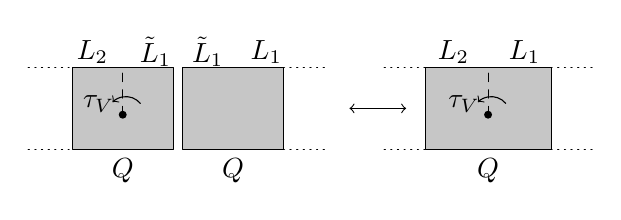
\begin{tikzpicture}[line cap=round,line join=round,scale=0.8]
\draw[dotted] (-0.7,1.3) -- (0,1.3);
\draw[dotted] (-0.7,0) -- (0,0);
\draw[fill=gray!45] (0,0) rectangle (1.6,1.3);
\draw[fill=gray!45] (1.75,0) rectangle (3.35,1.3);
\fill (0.8,0.55) circle (1.8pt);
\draw[dashed] (0.8,0.55) -- (0.8,1.3);
\draw[->] (1.08,0.73) arc[start angle=40,end angle=135,radius=0.3];
\node at (0.42,0.72) {$\tau_V$};
\node at (0.32,1.55) {$L_2$};
\node at (1.32,1.55) {$\tilde{L}_1$};
\node at (2.15,1.55) {$\tilde{L}_1$};
\node at (3.08,1.55) {$L_1$};
\node at (0.8,-0.34) {$Q$};
\node at (2.55,-0.34) {$Q$};
\draw[dotted] (3.35,1.3) -- (4.0,1.3);
\draw[dotted] (3.35,0) -- (4.0,0);
\draw[<->] (4.4,0.65) -- (5.3,0.65);
\draw[dotted] (4.95,1.3) -- (5.6,1.3);
\draw[dotted] (4.95,0) -- (5.6,0);
\draw[fill=gray!45] (5.6,0) rectangle (7.6,1.3);
\fill (6.6,0.55) circle (1.8pt);
\draw[dashed] (6.6,0.55) -- (6.6,1.3);
\draw[->] (6.88,0.73) arc[start angle=40,end angle=135,radius=0.3];
\node at (6.22,0.72) {$\tau_V$};
\node at (6.05,1.55) {$L_2$};
\node at (7.18,1.55) {$L_1$};
\node at (6.6,-0.34) {$Q$};
\draw[dotted] (7.6,1.3) -- (8.25,1.3);
\draw[dotted] (7.6,0) -- (8.25,0);
\end{tikzpicture}
\caption{}\label{fig:alpha-family}
\end{figure}
对 $l$ 与 $\tilde{l}$ 而言，同一种类型的论证有一个稍更复杂的版本也能奏效，其结果的形式为
\begin{equation*}
\boxed{\begin{aligned}
&\beta\colon CF^{\mathrm{pr}}(L_0,L_1)\otimes CF^{\mathrm{pr}}(Q,L_0)\longrightarrow CF^{\mathrm{pr}}(Q,L_2),\\
&\mu^1(\beta(\cdot,\cdot))+\beta(\mu^1(\cdot),\cdot)+\beta(\cdot,\mu^1(\cdot))\\
&\quad+\tilde{l}(b(\cdot),\cdot)+l(\cdot,\cdot)+\alpha(\mu^2(\cdot,\cdot))+\tilde{d}(h(\cdot,\cdot))=0.
\end{aligned}}
\end{equation*}
把它们合在一起，便得到一个\trChainMap
\begin{equation}\label{eq:chain-map-alpha-beta}
\begin{pmatrix}
b\otimes\mathrm{Id} & & \\
h & a & \\
\beta & \alpha & \mathrm{Id}
\end{pmatrix}
\colon D\longrightarrow\tilde{D}.
\end{equation}
\eqref{eq:chain-map-alpha-beta} 中的对角项都是\trContinuationMap，从而是\trQuasiisomorphism，所以整体仍将是一个\trQuasiisomorphism。最后，一个类似的论证表明：当 $L_2$ 作\trIsotopy{}时，$D$ 在\trQuasiisomorphic{}的意义下保持不变；为避免重复，我们略去这一部分。
